\section{Current Experimental Measurements}\label{sec:current}
Several experimental groups are currently investigating transition form factors in the time-like regime, including, but not limited to;
\begin{itemize}
	\item TRIUMF $\pi^0 \to \epem \gamma$~\cite{FARZ} 
	\item A2 Collaboration $\eta \to \epem \gamma$~\cite{Berg,A2} 
	\item Multiple Groups $\omega\to\pi^0 \mu^+\mu^-$ ~\cite{Dzhelyadin:1980tj,Arnaldi:2009aa,Uras:2011zz}
	\item CLEO Collaboration $\eta'\to e^+e^-\gamma $~\cite{CLEO}
	\item Lepton-G $\eta'\to \mu^+\mu^-\gamma $~\cite{DZH}
	\item BESIII Collaboration $\eta'\to e^+e^-\gamma $~\cite{Ablikim:2015wnx}
	\item KLOE Collaboration $\phiDalT$~\cite{Babusci:2014ldz} .
\end{itemize}
The branching ratio of \etaPDal \ remained an upper limit, Fig.~\ref{fig:past}, until the BESIII collaboration finally measured it using 1.31 billion $J/\psi \to \gamma \etaP \to \gamma \gamma \epem$. From the BESIII data sample, Fig.~\ref{fig:past}, only 894 \etaPDal \ events were recorded which lead to a determination of the branching ratio $\Gamma_{\eta^{\prime} \rightarrow e^+e^- \gamma}  = 4.69 \pm 0.2 (\mathrm{stat.})\cdot 10^{-4}$ and a slope parameter, Eq.~\ref{eq:tffslope}, $b = 1.60\pm0.17(\mathrm{stat.}$ which is consistent with the measurement from Lepton-G ($1.7 \pm 0.4 (\mathrm{stat.}$). The slope parameter measured by BESIII and Lepton-G, which is the essential measurement needed for the HLbl contribution, is not sufficient to distinguish between different theoretical approaches listed in ~\ref{tab:theory}. Some of the obstacles for not measuring the \etaPDal \ was the low branching ratio, pion contamination and low electron PID efficiency. These obstacles will be mitigated with CLAS12 because of the luminosity, cross-section for exclusive $\etaP$ production and superior \epemT/\pipiT rejection of $\lesssim 10^{10}$. 

%The experiential results of the $\pi^0$ and $\omega$ present a puzzle because for the $\pi^0$ the measurement in the time-like region does not have agreement between several experiemtn
%
%The experimental results on the conversion decay of the $\omega$ meson, $\omega\to\pi^0 \mu^+\mu^-$  present a puzzle ~\cite{Dzhelyadin:1980tj,Arnaldi:2009aa,Uras:2011zz}. 
%The measurements suggest a dramatic increase of the transition form factor for large momentum transfers that is not consistent with VMD models nor explicable with modern theoretical advances. 
%These experimental results are in contradiction to measurements in the space-like regime~\cite{Achasov:2013btb}. 
%The situation makes it important to investigate the conversion decays of vector mesons. 
%
%{\it ... mention A2 measurement ? ...}
%
%The conversion decays of the  $\omega$ meson are currently being studied within the LMD group using data from the CLAS g12 experiment. 
%We plan to approach the conversion decays of the $\phi$ meson by analyzing the decay $\phi\to\eta\gamma^\star$ based on the proposed experiment. 
%The decay $\phi \to \pi^0\gamma^\star$ would enable access to higher dilepton masses and more precise mapping of transition form factors in this kinematic regime. However, the decay is OZI suppressed and statistically significant results may be obtained after a luminosity upgrade of the experiment facility.
%Current measurements by the KLOE collaboration for $\phi\to\eta e^+e^-$~\cite{Babusci:2014ldz} and $\phi\to\pi^0 e^+e^-$~\cite{Anastasi:2016bfh} have improved the values for the respective branching ratios by the SND and CMD-2 collaborations ~\cite{Achasov:2000ne,Akhmetshin:2000bw,Achasov:2002hs,Akhmetshin:2000wi}. The $\phi\to\eta e^+e^-$ measurement by KLOE is based on ~31000 events and deduces a slope parameter of $ \text{KLOE} \ b_{\phi\eta}=1.28\pm 0.10^{+0.09}_{-0.08} $.
%
%{\it ... figure of KLOE phi-eta TFF here? ...}
\begin{figure}[h!]\begin{center}
		\subfloat[$\phi$ Dalitz and conversion spectra from g12][]{ %Feynman diagram of $\etaP$ Dalitz decay
			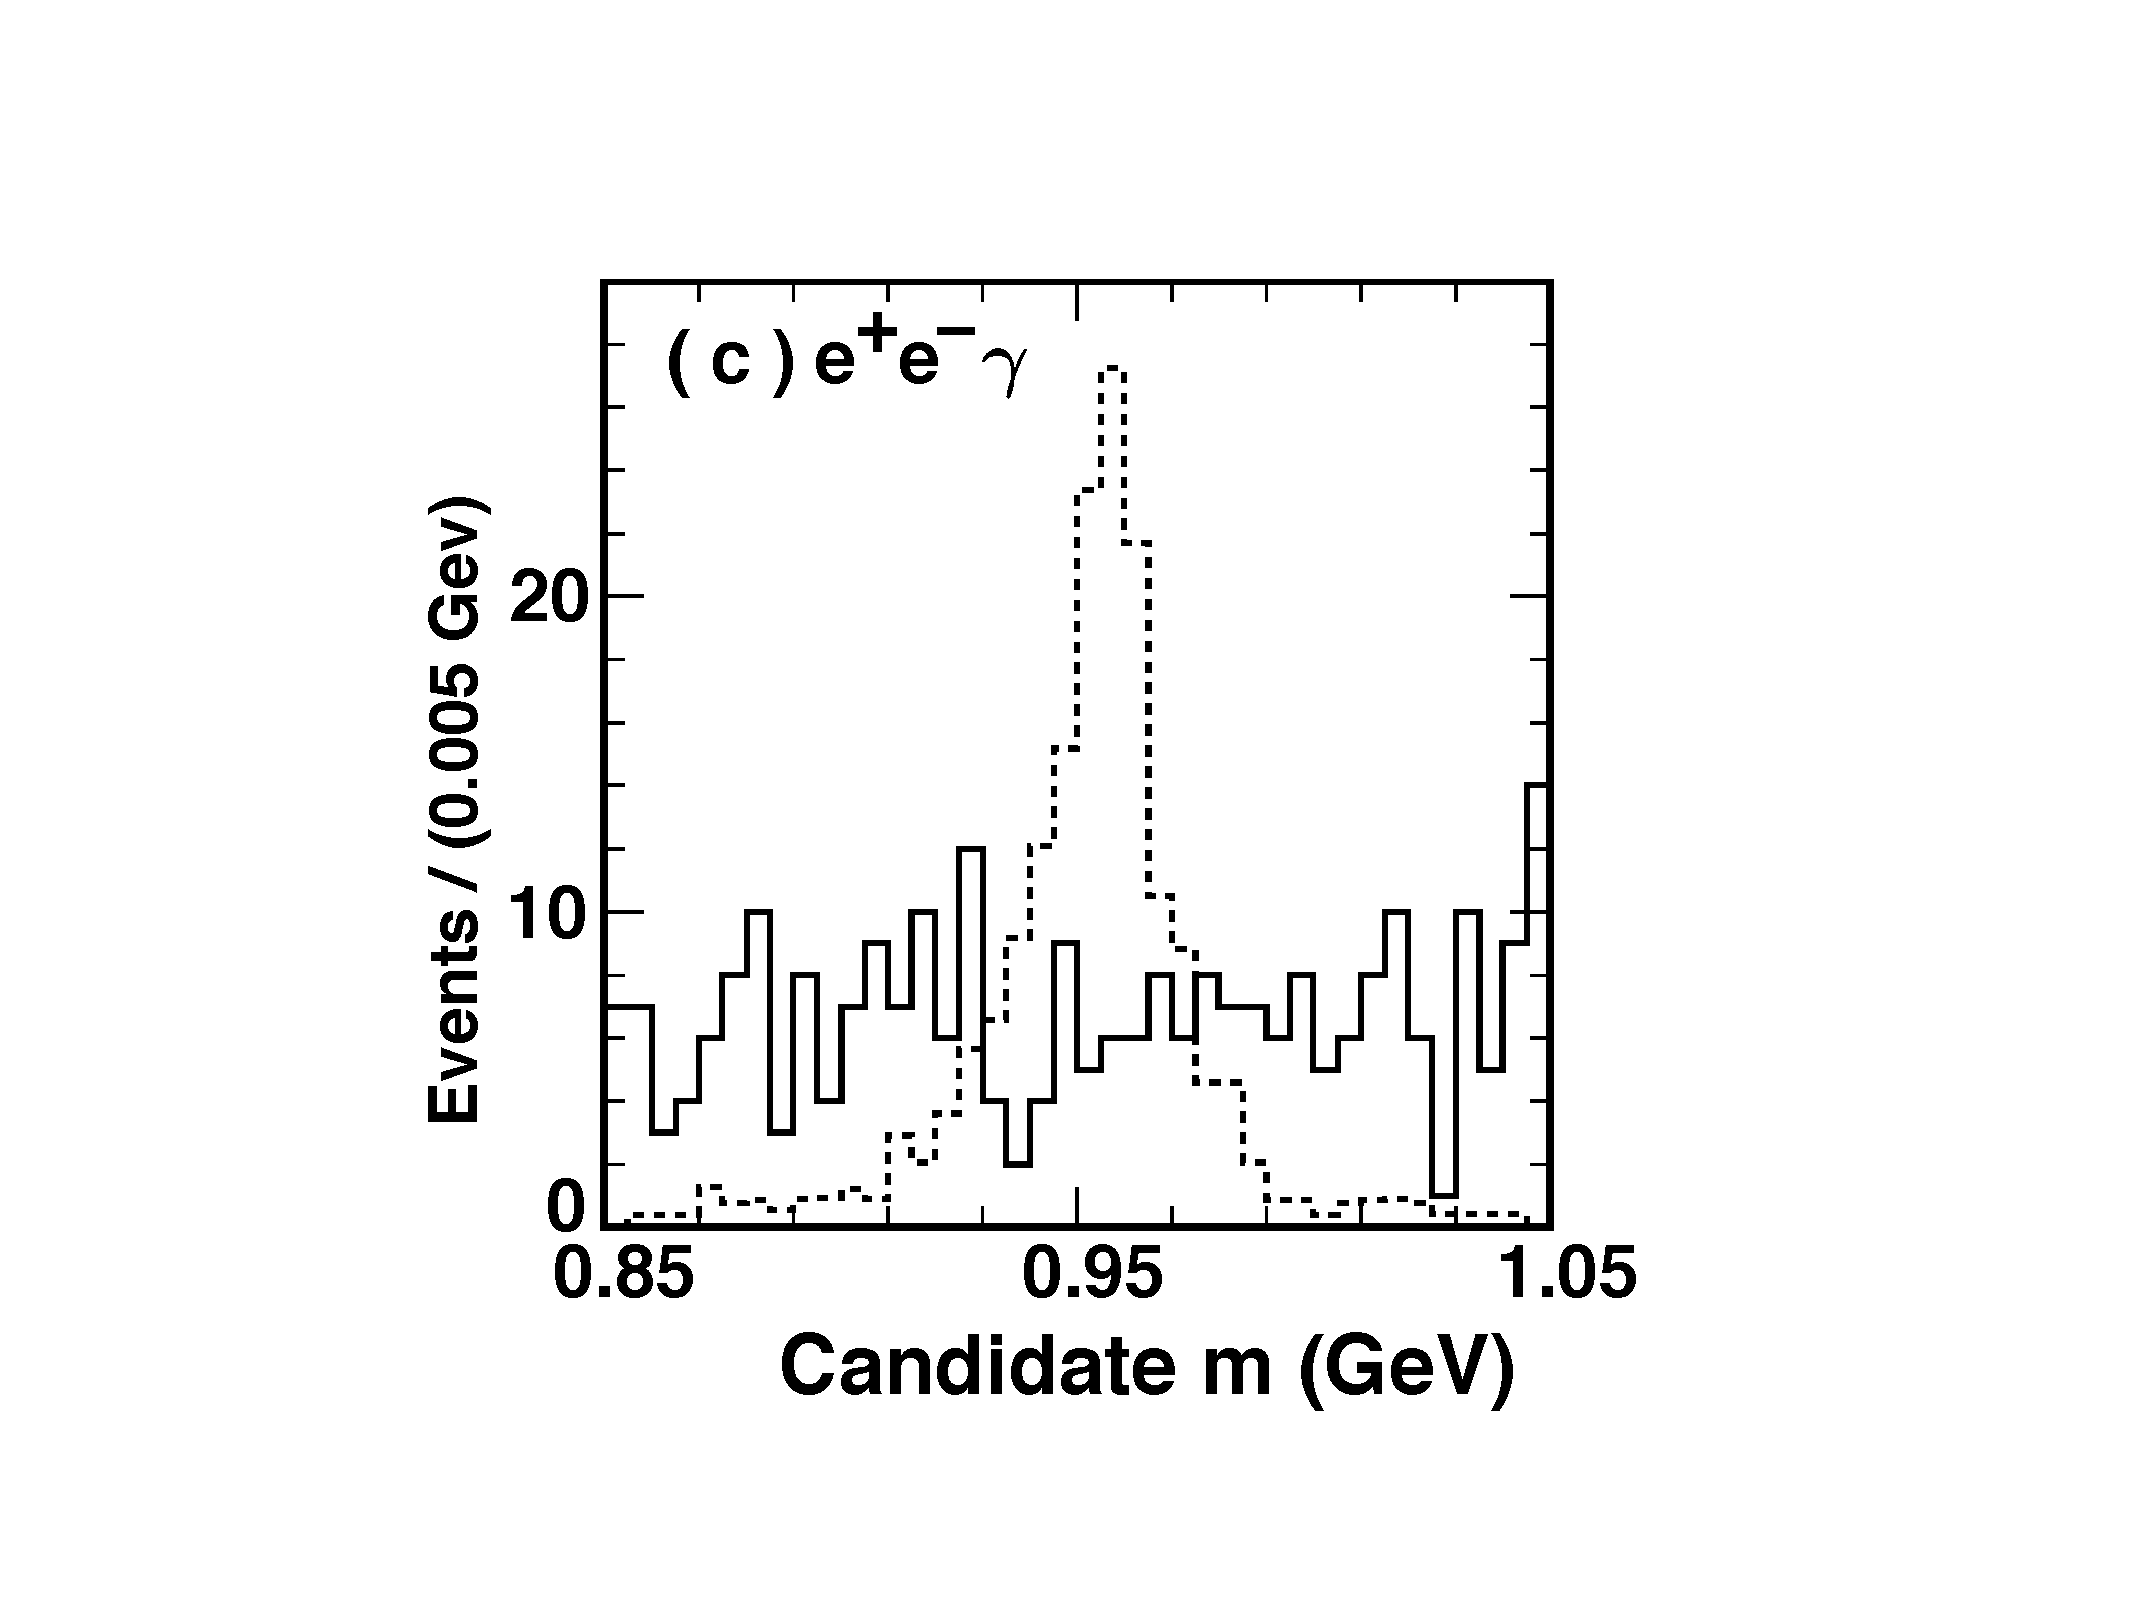
\includegraphics[width=1.0\columnwidth,height=1.0\qfigheight]{\grpath/current_status/CLEO_keynote.pdf}\label{fig:CLEO}
		}
		\\
		\subfloat[$\etaP$ Dalitz and conversion spectra from BESIII][]{ %Feynman diagram of $\etaP$ two photon decay
			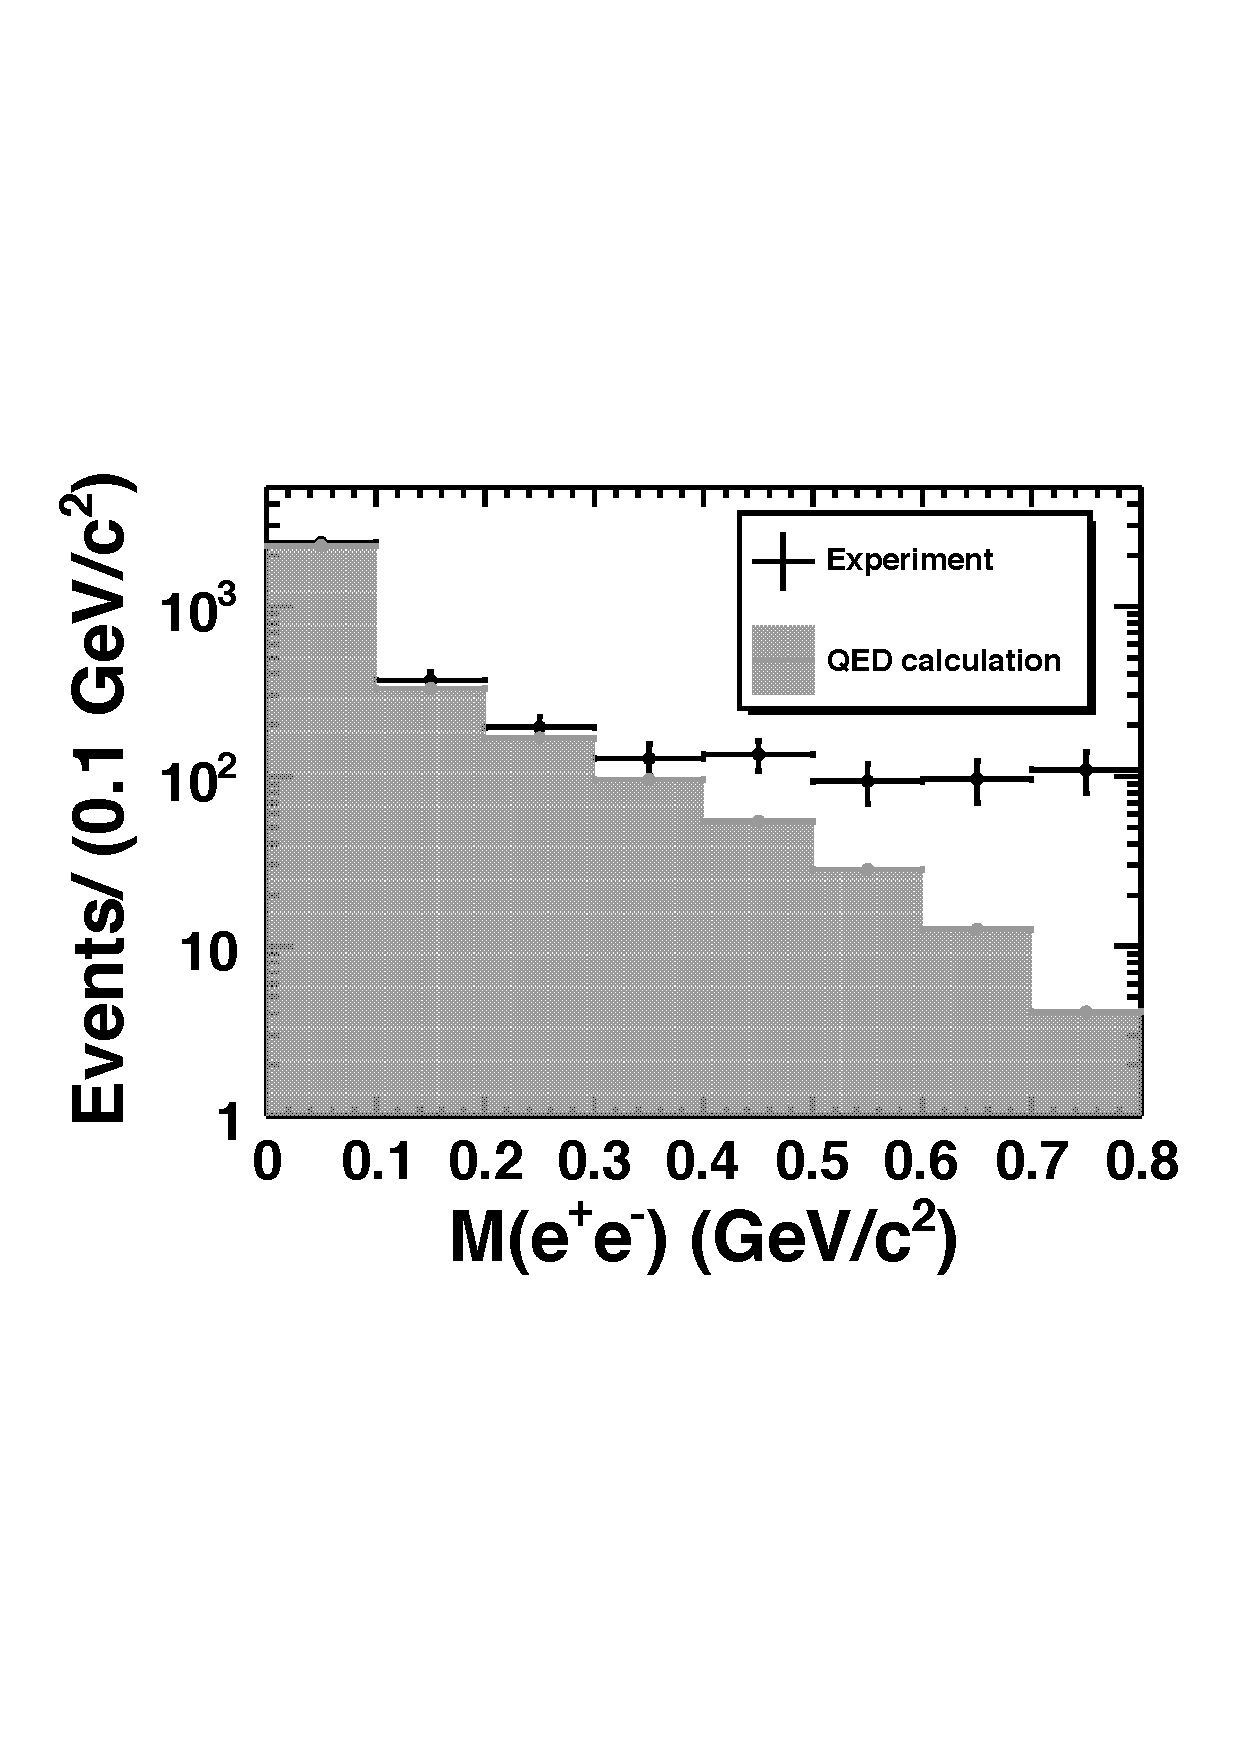
\includegraphics[width=0.8\columnwidth,height=1.8\qfigheight]{\grpath/current_status/BESIII_EtaP.pdf}\label{fig:BESIII}
		}
		\caption[Counts rates for \etaTP from previous experiements]{\label{fig:past} ~\subref{fig:CLEO} Missing mass off of the proton for \etaPDal \ from the CLEO collaboration~\cite{CLEO}, solid line(data), dashed(MC expectation).~\subref{fig:BESIII}Counts of $M(\epem)$ from the first published observation of the \etaPDal \  by BESIII~\cite{BESIII}. }
\end{center}\end{figure}
	\FloatBarrier 	
	\subsection{Previous CLAS analyses}
	The LMD (Light Meson Decay) group of CLAS was established to investigate the decay properties of light mesons. Two experiments in CLAS are currently being analyzed in the LMD group. The g12 experiment, performed with CLAS, is one experiment chosen due to its ability to identify leptons with the use of the Cherenkov detectors (CC).
	% performed with the g12 experiment
	The g12 experiment produced a data set of photon-induced reactions. Fortunately, the Cherenkov Counters were filled with perflourbutane ($C_4F_{10}$) and a trigger consisting of a coincidence between the (ST$\cdot$TOF)(CC$\cdot$EC) allowing the study of dilepton reactions throughout the entire beam energy range $1.15 \ \mathrm{GeV}<E_\gamma <5.45 \ \mathrm{GeV}$. The g12 experiment ran for 44 days however, the trigger that allowed for \epemT identification was established for $\sim$29 days of beam-time. Using approved dilepton identification~\cite{g12note}, preliminary analyses of g12 involving dileptons include the decays:
	\begin{itemize}
		\item $\Delta \to p \epem$ (Transition form factor)
		\item $\eta \to \epem \gamma$ (Transition form factor)
	\end{itemize}
	while advanced analyses involving dileptons include:
	\begin{itemize}
		\item $\piz \to \epem \gamma$ (Differential Cross-Section)
		\item $\omega / \rho \to \epem$ (Interference of $\omega/\rho$ )
		\item $\omega \to \epem \piz$ (Transition form factor)
		\item $\etaP \to \epem \gamma$ (Transition form factor / branching ratio)
	\end{itemize}
	The g12 \etaPDal \ analysis provided CLAS its first look at the possibility of measuring the branching ratio and transition form factor. Using the Qfactor, signal to background separation, technique derived in CLAS~\cite{qfactor}, the total count rate of \etaPDal \ events detected in g12 was $\sim 89$. Figure~\ref{fig:g12figs} depicts the $\etaP$ signal extracted in g12 along with the $M(\epem)$ spectrum from the signal. 
	\begin{figure}[h!]\begin{center}
			\subfloat[$\etaP$ Dalitz and conversion spectra from g12][]{ %Feynman diagram of $\etaP$ two photon decay
				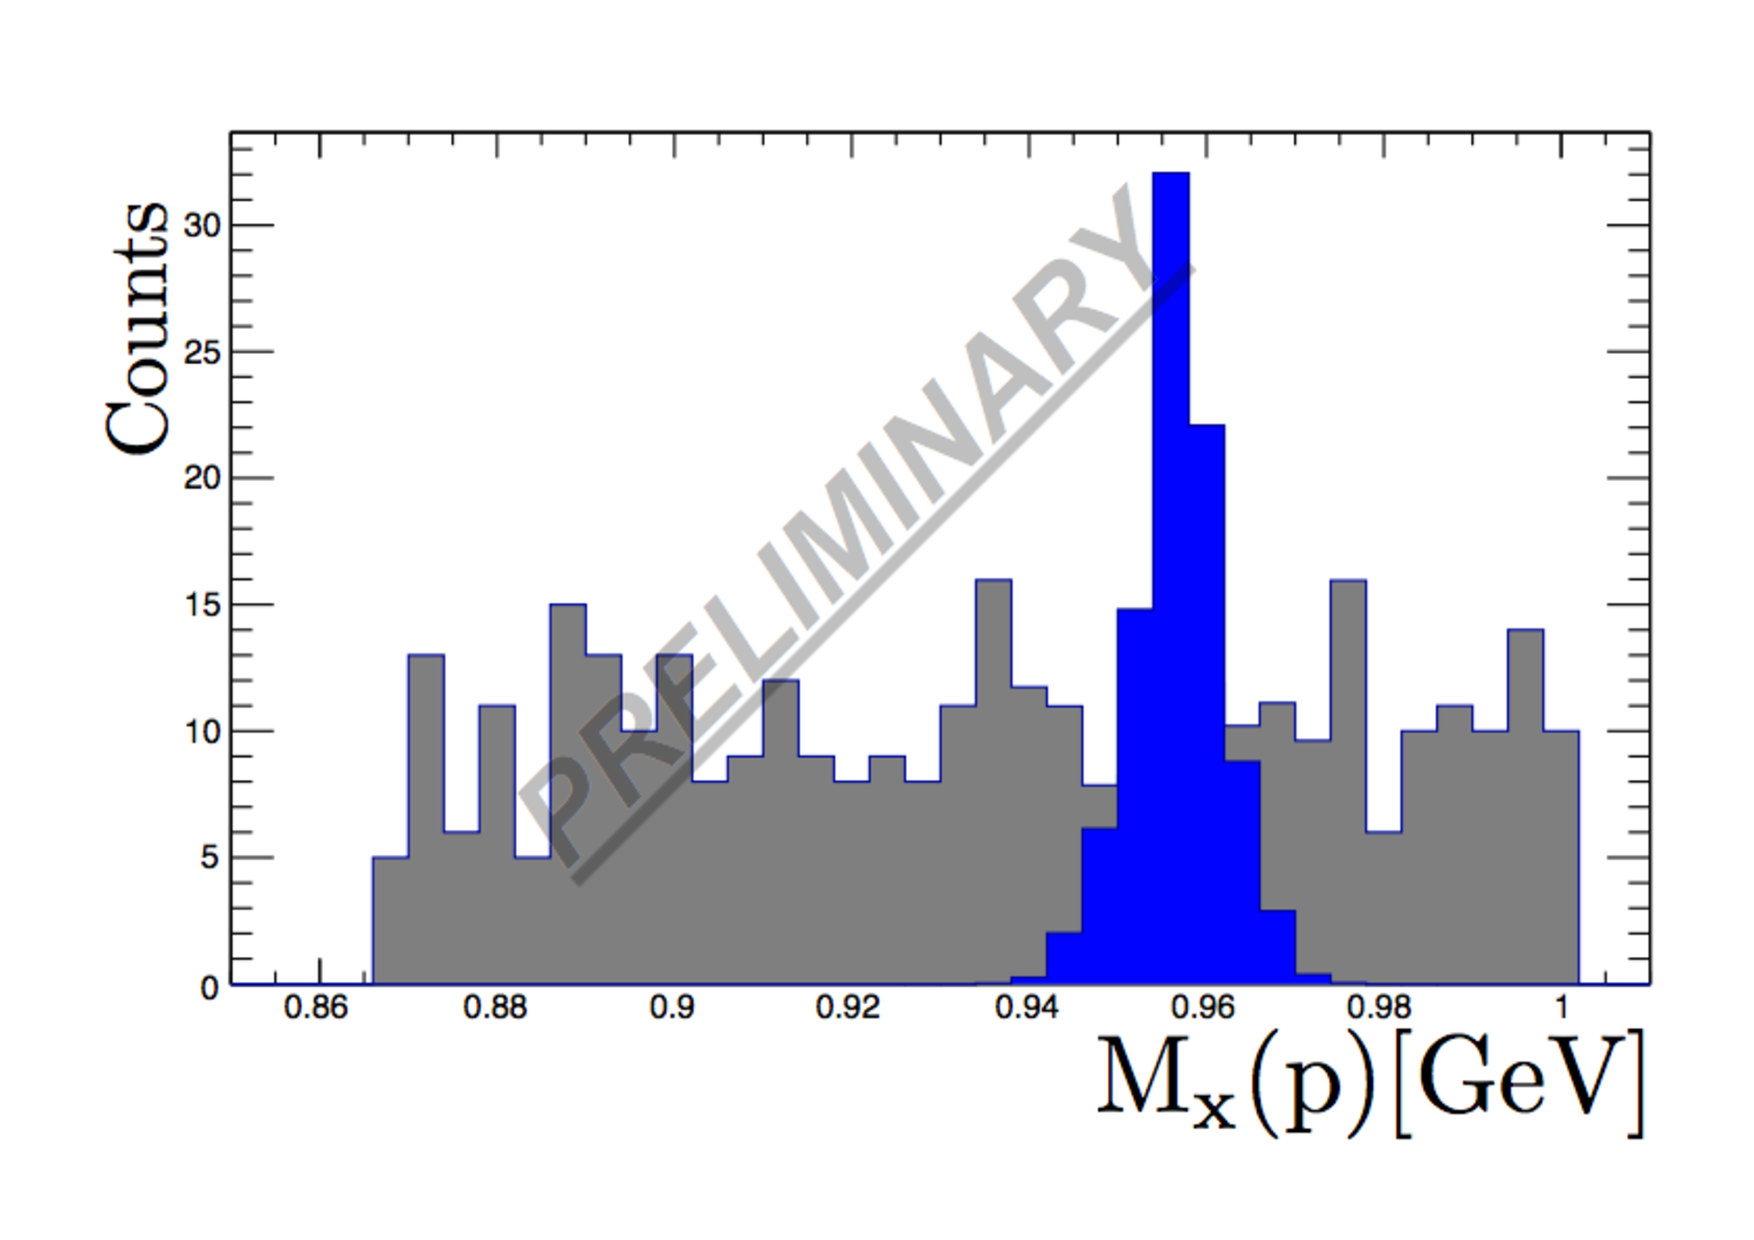
\includegraphics[width=0.8\columnwidth,height=1.0\qfigheight]{\grpath/g12/MxP_g12.pdf}\label{fig:g12MxP}
			}
			\\
			\subfloat[$\phi$ Dalitz and conversion spectra from g12][]{ %Feynman diagram of $\etaP$ Dalitz decay
				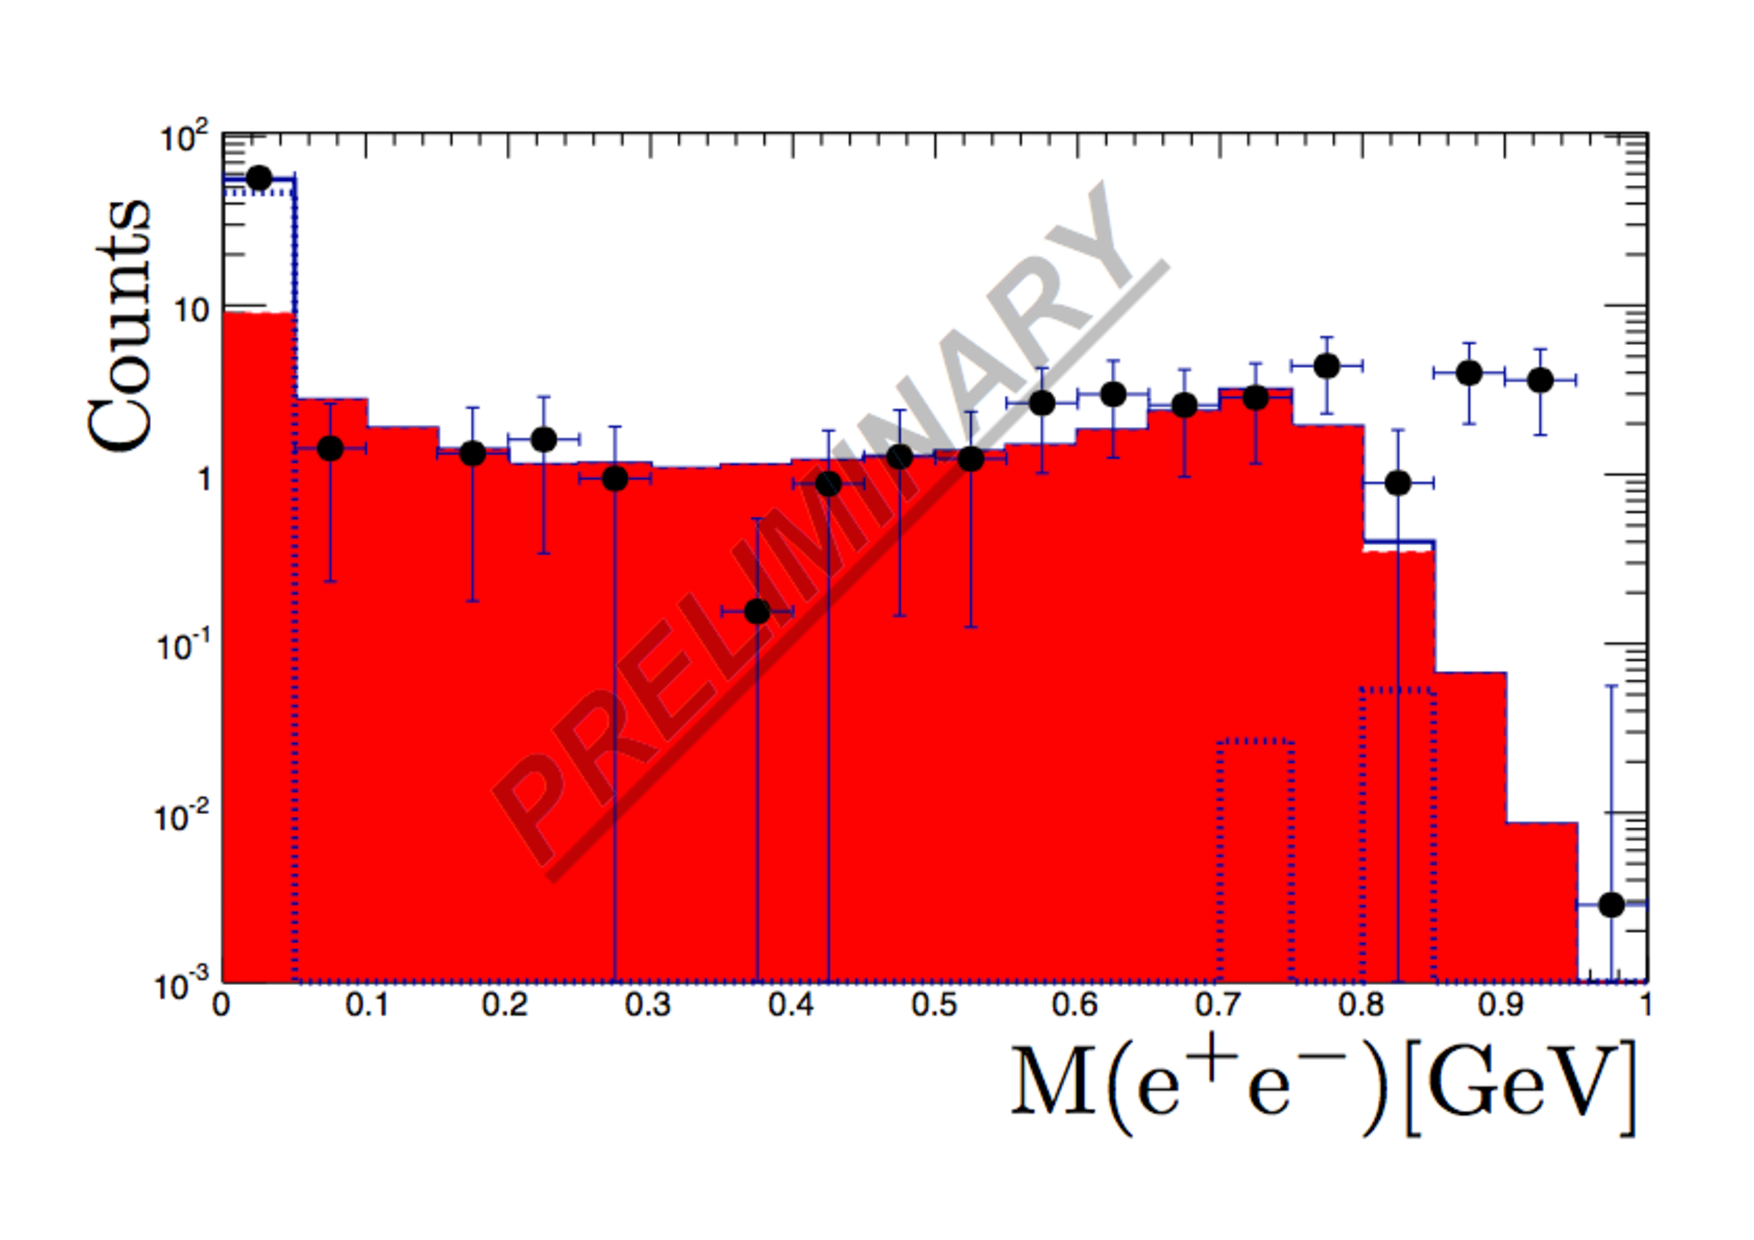
\includegraphics[width=0.8\columnwidth,height=1.0\qfigheight]{\grpath/g12/EpEm_g12.pdf}\label{fig:g12EpEm}
			}
			\caption[Counts rates for \etaTP from g12]{\label{fig:g12figs}~\subref{fig:g12MxP} Missing mass off of the proton for \etaPDal \  from CLAS g12. Q-factor weighted(Blue), Background (Grey). ~\subref{fig:g12EpEm} Invariant mass spectrum of \epemT \ under the blue curve in~\subref{fig:g12MxP}. Total counts in 29 days $\sim$ 89.}
		\end{center}\end{figure}
		\FloatBarrier 	
		As seen in Fig.~\ref{fig:g12figs} the current CLAS results suffer from insufficient statistics. Therefore, we propose to repeat the \etaPDal \  measurement with CLAS12.
		\FloatBarrier